\documentclass[a4paper,12pt]{article}

\usepackage{ucs}
\usepackage[utf8x]{inputenc}
\usepackage{amsmath}
\usepackage{amsfonts}
\usepackage{amssymb}
\usepackage{amsthm}
\usepackage{fontenc}
\usepackage{graphicx}
\usepackage{booktabs}
\usepackage[left=2cm, right=2cm, top=1.5cm, bottom=1.5cm]{geometry}
\title{COMP8650 Assignment 6}
\author{Ragib Zaman u6341578}

\newcommand{\bi}[2]{ \binom{#1}{#2}  }
\newcommand{\p}{\prod}
\newcommand{\e}{\mathbf{e}}

\begin{document}
\maketitle


\paragraph{Q1 - Conv2d and ConvTranspose2d}
\
\newline

\paragraph{a)}
\
For a Conv2d layer, we have the following relation between $H_{in}$ and $H_{out}$ -

$$ H_{out} =\bigg\lfloor \frac{ H_{in} + 2 \cdot \text{padding} - \text{kernel\_size} }{ \text{stride} } + 1\bigg\rfloor$$
The same relation also holds with $W$ in place of $H.$ In this case, we have $H_{in} = W_{in} = 64,$ $\text{kernel\_size} = 3, \ \text{stride} = 1$ and $\text{padding}=1$ so we have

$$ H_{out} = W_{out} = \bigg\lfloor \frac{ 64 + 2 \cdot 1 - 3 }{ 1 } + 1\bigg\rfloor = 64$$
So the size of the output for the Conv2d layer is
$$(N, C_{out}, H_{out}, W_{out} ) = (32, 16, 64, 64)$$
\paragraph{b)}
\
For a ConvTranspose2d layer, we have the following relation between $H_{in}$ and $H_{out}$ -

$$ H_{out} = (H_{in}-1)\cdot \text{stride} - 2\cdot \text{padding} + \text{kernel\_size}$$
The same relation also holds with $W$ in place of $H.$ In this case, we have $H_{in} = W_{in} = 1,$ $\text{kernel\_size} = 3, \ \text{stride} = 1$ and $\text{padding}=0$ so we have

$$ H_{out} = W_{out} = (1-1)\cdot 1 - 2\cdot 0 + 3 = 3$$
So the size of the output for the ConvTranspose2d layer is
$$(N, C_{out}, H_{out}, W_{out} ) = (32, 128, 3, 3)$$
\paragraph{c)}
\
This question is done similarly to part b), but in this case we have $H_{in} = W_{in} = 31,$ $\text{kernel\_size} = 5, \ \text{stride} = 2$ and $\text{padding}=0$ so we have

$$ H_{out} = W_{out} = (31-1)\cdot 2 - 2\cdot 0 + 5 = 65$$
So the size of the output for the ConvTranspose2d layer is
$$(N, C_{out}, H_{out}, W_{out} ) = (32, 32, 65, 65)$$

\paragraph{d)}
\
In a Conv2d layer we learn a weight tensor which has dimension $$(C_{out}, C_{in}, \text{kernel\_size[0]},\text{kernel\_size[1]})$$
In this case we have $C_{out} = 16, C_{in} = 3, \text{kernel\_size[0]}=\text{kernel\_size[1]}=3$ so the number of parameters in the weight tensor is $ 16 \cdot 3 \cdot 3 \cdot 3 = 432.$ We also learn a bias vector which has size $C_{out} = 16.$ So the total number of learnable parameters in the Conv2d layer is $448.$ 
\paragraph{Q3 - Experiments}
\
\newline

\paragraph{a), b)}
\
The model layers are indeed correctly sized. The asgn6.py script runs, results for 500 and 10,000 epochs saved in 5layers\_500epochs and 5layers\_10000epochs respectively. 
\paragraph{c)}
\
Below we have plot the Loss vs Iterations over 500 epochs on linear and log scales respectively. While the linear scale plot may make it appear that we have essentially converged, the log scale plot makes it more apparent that we could probably achieve noticeably better results if we train for more epochs.
\newline
\includegraphics[scale=0.5,keepaspectratio=true]{../asgn6starter/5layer_500epoch/loss_linear.png}
% loss_linear.png: 0x0 pixel, 0dpi, nanxnan cm, bb=
\includegraphics[scale=0.5,keepaspectratio=true]{../asgn6starter/5layer_500epoch/loss_log.png}
\newline
Below we have the same information as above, but after 10,000 epochs. This now appears much closer to convergence than at 500 epochs.
\newline
\includegraphics[scale=0.5,keepaspectratio=true]{../asgn6starter/5layer_10000epoch/loss_linear.png}
% loss_linear.png: 0x0 pixel, 0dpi, nanxnan cm, bb=
\includegraphics[scale=0.5,keepaspectratio=true]{../asgn6starter/5layer_10000epoch/loss_log.png}

\paragraph{d)}
\
The images below show denoised samples after 500 epochs and 10,000 epochs respectively. More samples can be found in the folders 5layers\_500epochs and 5layers\_10000epochs. The general shape of the target image is accurately determined quite early in the training (e.g. after 1000 iterations). At about 500 epochs we can start to see more features of the Pokemon such as eyes, but the images are quite noticeably blurry. By 10,000 epochs the quality of the denoised samples has greatly improved, looking almost indistinguishable from the target image. There are still some imperfections however, such as failing to recreate thin lines (e.g. see the Magikarp). 
\begin{center}
 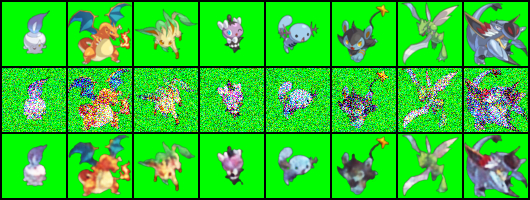
\includegraphics[scale=0.9,keepaspectratio=true]{../asgn6starter/5layer_500epoch/sample-003500.png}
 % sample-003500.png: 0x0 pixel, 0dpi, 0.00x0.00 cm, bb=
\end{center}
\begin{center}
 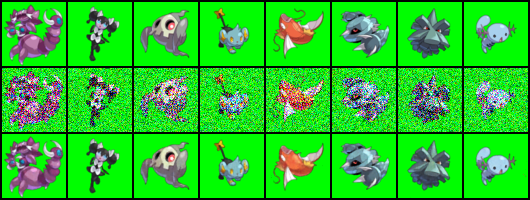
\includegraphics[scale=0.9,keepaspectratio=true]{../asgn6starter/5layer_10000epoch/sample-070000.png}
 % sample-070000.png: 0x0 pixel, 0dpi, nanxnan cm, bb=
\end{center}

\paragraph{e)}
\
The images below show samples generated from a random noise input after 500 epochs and 10,000 epochs respectively. More samples can be found in the folders 5layers\_500epochs and 5layers\_10000epochs. After 1000 iterations, the samples simply look like colourful blobs. As training continues they behin to take shapes seeming more similar to typical Pokemon. By 10,000 epochs, the samples are often recognised as similar to Pokemon by people who squint and look from far away (I tested this on a few friends). 
\begin{center}
 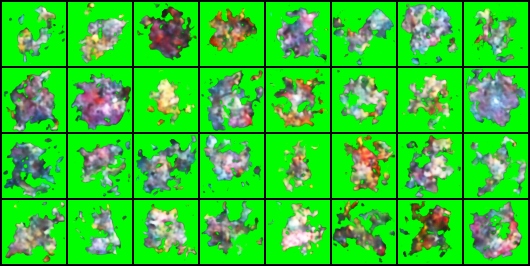
\includegraphics[scale=0.9,keepaspectratio=true]{../asgn6starter/5layer_500epoch/novel-003500.png}
 % sample-003500.png: 0x0 pixel, 0dpi, 0.00x0.00 cm, bb=
\end{center}
\begin{center}
 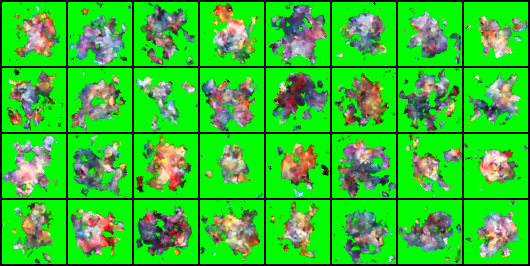
\includegraphics[scale=0.9,keepaspectratio=true]{../asgn6starter/5layer_10000epoch/novel-070000.png}
 % sample-070000.png: 0x0 pixel, 0dpi, nanxnan cm, bb=
\end{center}
\paragraph{e)}
\
All experiments in this section were trained for 500 epochs. Python source and sample images can be found in the zip file. 
\paragraph{Number of layers in Decoder}- In addition to the 5 layer decoder specified in the assignment, I created Decoders with 1,2,3,4 and 6 layers. The 1-layer decoder is particularly interesting: the novel samples seem almost like random noise, with some pattern around the borders of the image. Despite this seeming a lot less like Pokemon than the novel samples for e.g. the 5 layer decoders, the denoised samples are surprisingly good. They are in fact not as blurry as the 5 and 6 layer decoders are after 500 epochs. The lack of smoothing is noticeable in the prescence of blemish type artifacts on the images however. The 6 layer decoder produces very blurry images after 500 epochs, and I would expect this problem to get worse with more layers without adding more data and training time. 
\paragraph{Final activation functions}- In the assignment specification, the final activation function for the encoder and the decoder was Tanh. Replacing this with ReLU and Sigmoid resulted in images where dark areas became very dark. I conjectured that this was because ReLU and Sigmoid have only non-negative outputs and that dark areas need negative outputs to be represented well. Using the PReLU activation, which can take negative values, goes back to producing more normal images like we had with Tanh. 
\paragraph{Latent Size}- In addition to the assignments default latent size of 128, I tried 32 and 256. With a latent size of 32, the denoised samples seem noticeably more blurry than the default case, which seems intuitive (less latent features make it harder to encode fine details). Somewhat surprisingly, with a latent size of 256 the images also seem more blurry than the default case. This may be a case of simply requiring more training time as we have more learnable parameters.
\paragraph{Large Kernel Size}- In this experiment I simply increased the kernel sizes of the decoder specified in the assignment. As expected, the denoised samples become more blurry. The novel samples also appear to be more concentrated into fewer pieces near the middle of the image. 
\end{document}
